\documentclass{standalone}
\usepackage{tikz}
\usetikzlibrary{patterns, positioning}
\usepackage[sfdefault]{ClearSans} %% option 'sfdefault' activates Clear Sans as the default text font
\usepackage[T1]{fontenc}

\begin{document}
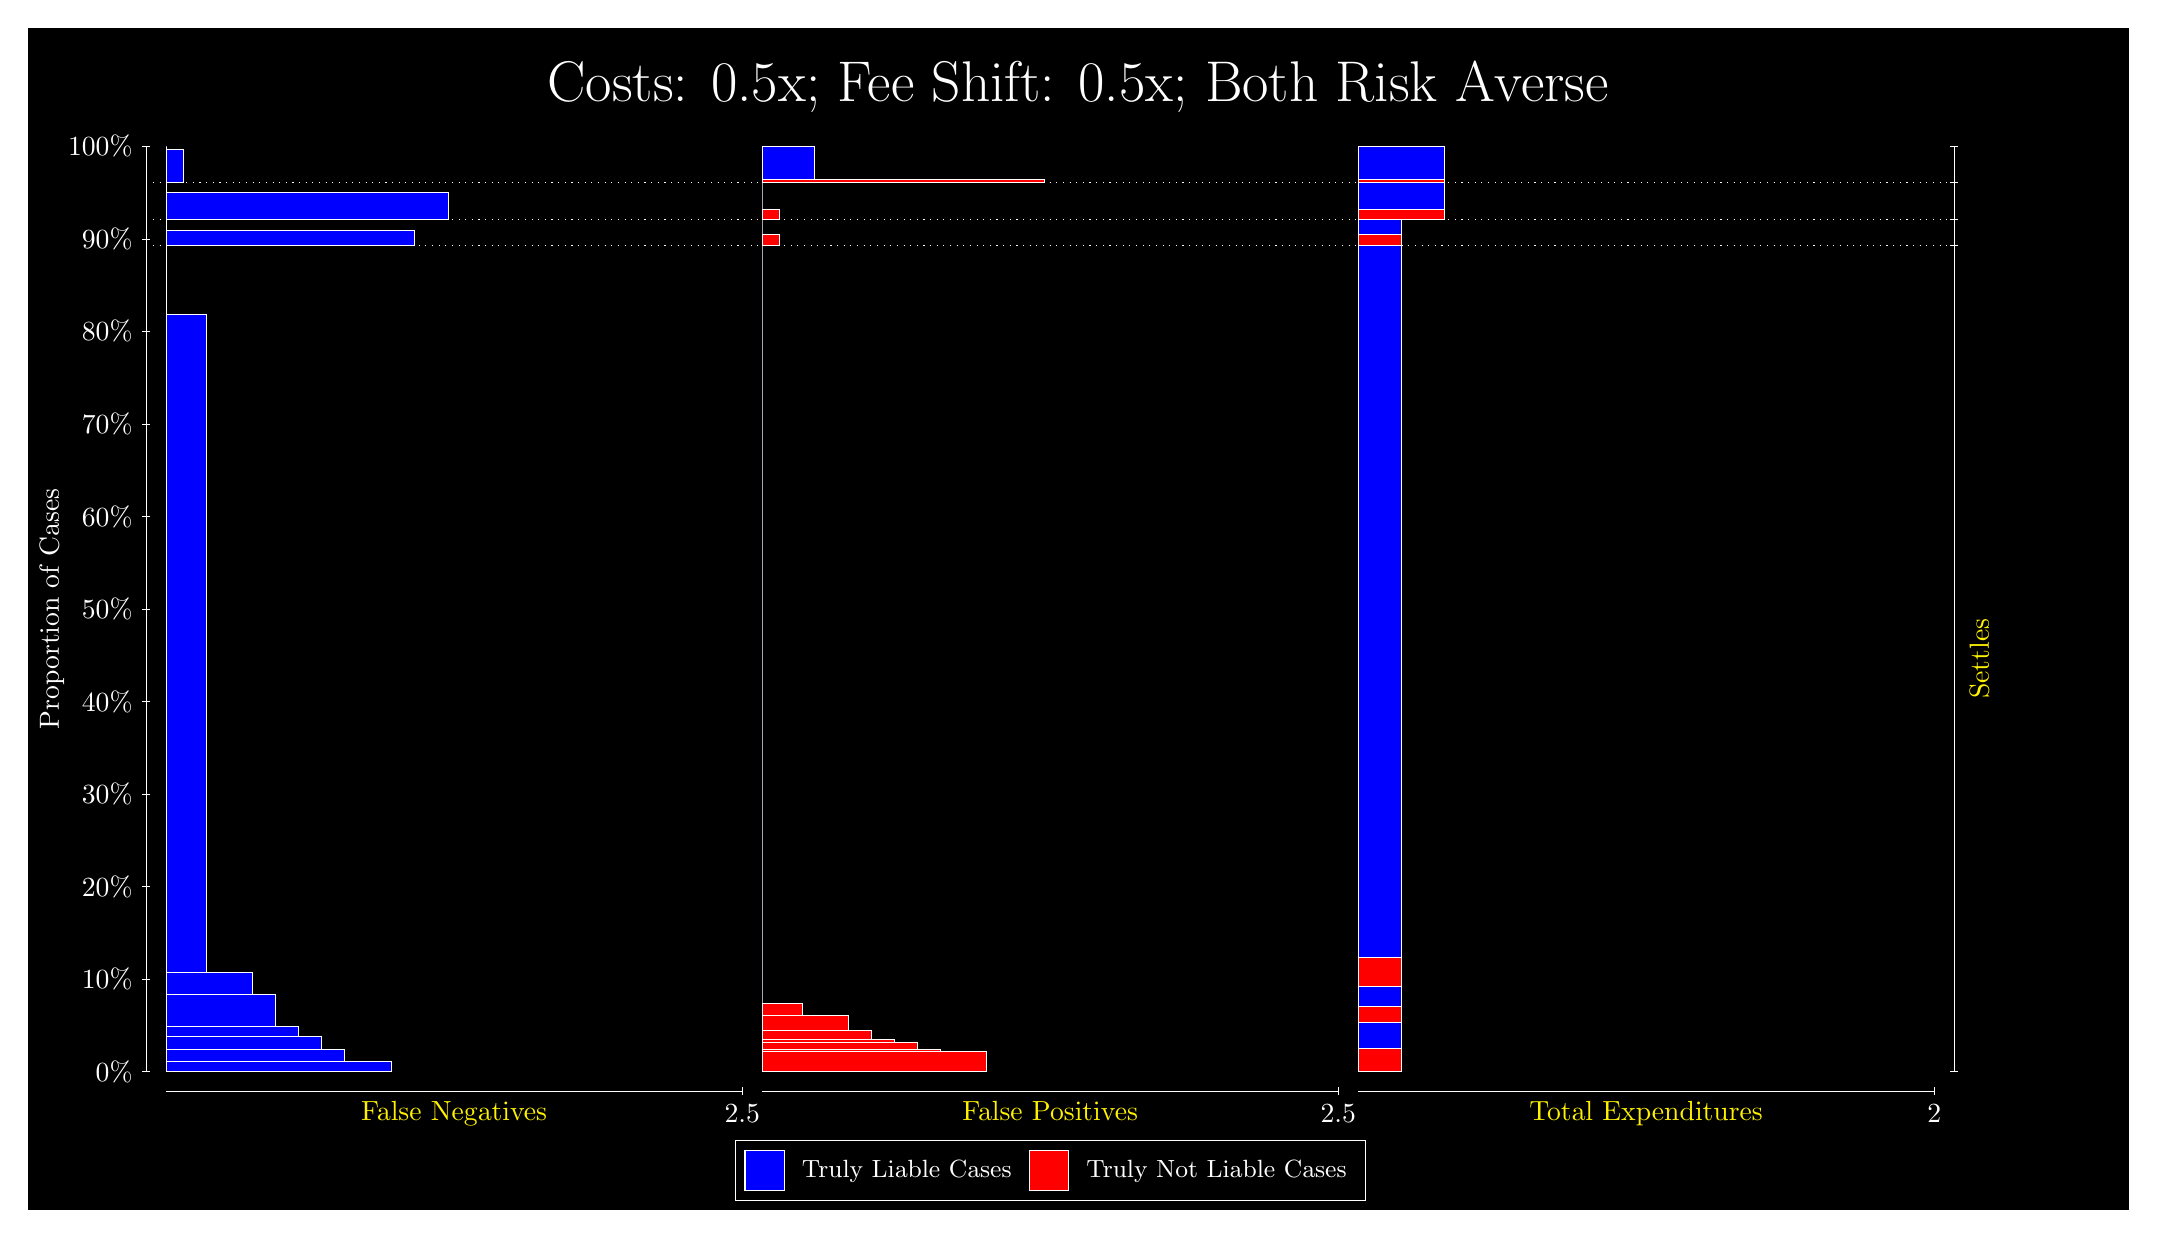
\begin{tikzpicture}
\draw[fill=black] (0,0) rectangle (26.667,15);
\draw[text=white] (0,13.5) rectangle (26.667,15) node[midway] {\huge Costs: 0.5x; Fee Shift: 0.5x; Both Risk Averse};
\draw[white, very thin] (1.5,1.75) -- (1.5,13.5);
\node[rotate=90, text=white, anchor=center] at (0.3, 7.625) {Proportion of Cases};
\draw[white, very thin] (1.45,1.75) -- (1.55,1.75);
\node[text=white, anchor=east] at (1.45, 1.75) {0\%};
\draw[white, very thin] (1.45,2.925) -- (1.55,2.925);
\node[text=white, anchor=east] at (1.45, 2.925) {10\%};
\draw[white, very thin] (1.45,4.1) -- (1.55,4.1);
\node[text=white, anchor=east] at (1.45, 4.1) {20\%};
\draw[white, very thin] (1.45,5.275) -- (1.55,5.275);
\node[text=white, anchor=east] at (1.45, 5.275) {30\%};
\draw[white, very thin] (1.45,6.45) -- (1.55,6.45);
\node[text=white, anchor=east] at (1.45, 6.45) {40\%};
\draw[white, very thin] (1.45,7.625) -- (1.55,7.625);
\node[text=white, anchor=east] at (1.45, 7.625) {50\%};
\draw[white, very thin] (1.45,8.8) -- (1.55,8.8);
\node[text=white, anchor=east] at (1.45, 8.8) {60\%};
\draw[white, very thin] (1.45,9.975) -- (1.55,9.975);
\node[text=white, anchor=east] at (1.45, 9.975) {70\%};
\draw[white, very thin] (1.45,11.15) -- (1.55,11.15);
\node[text=white, anchor=east] at (1.45, 11.15) {80\%};
\draw[white, very thin] (1.45,12.325) -- (1.55,12.325);
\node[text=white, anchor=east] at (1.45, 12.325) {90\%};
\draw[white, very thin] (1.45,13.5) -- (1.55,13.5);
\node[text=white, anchor=east] at (1.45, 13.5) {100\%};

\draw[white, very thin] (24.457,1.75) -- (24.457,13.5);
\draw[white, very thin] (24.407,1.75) -- (24.507,1.75);
\node[anchor=west] at (24.407, 1.75) {};
\draw[white, very thin] (24.407,12.238) -- (24.507,12.238);
\node[anchor=west] at (24.407, 12.238) {};
\draw[white, very thin] (24.407,12.575) -- (24.507,12.575);
\node[anchor=west] at (24.407, 12.575) {};
\draw[white, very thin] (24.407,13.045) -- (24.507,13.045);
\node[anchor=west] at (24.407, 13.045) {};
\draw[white, very thin] (24.407,13.5) -- (24.507,13.5);
\node[anchor=west] at (24.407, 13.5) {};

\draw[white, very thin, fill=blue] (1.75,1.75) rectangle (4.6044,1.8743);
\draw[white, very thin, fill=blue] (1.75,1.8743) rectangle (4.0188,2.0266);
\draw[white, very thin, fill=blue] (1.75,2.0266) rectangle (3.7261,2.1968);
\draw[white, very thin, fill=blue] (1.75,2.1968) rectangle (3.4333,2.3231);
\draw[white, very thin, fill=blue] (1.75,2.3231) rectangle (3.1406,2.726);
\draw[white, very thin, fill=blue] (1.75,2.726) rectangle (2.8478,3.0151);
\draw[white, very thin, fill=blue] (1.75,3.0151) rectangle (2.2623,11.365);
\draw[white, very thin, fill=red] (1.75,11.365) rectangle (1.75,12.238);
\draw[white, very thin, fill=blue] (1.75,12.238) rectangle (4.8971,12.436);
\draw[white, very thin, fill=red] (1.75,12.436) rectangle (1.75,12.575);
\draw[white, very thin, fill=blue] (1.75,12.575) rectangle (5.3362,12.921);
\draw[white, very thin, fill=red] (1.75,12.921) rectangle (1.75,13.045);
\draw[white, very thin, fill=blue] (1.75,13.045) rectangle (1.9696,13.462);
\draw[white, very thin, fill=red] (1.75,13.462) rectangle (1.75,13.5);
\draw[white, very thin, fill=red] (9.3189,1.75) rectangle (12.173,2.0109);
\draw[white, very thin, fill=red] (9.3189,2.0109) rectangle (11.588,2.029);
\draw[white, very thin, fill=red] (9.3189,2.029) rectangle (11.295,2.1158);
\draw[white, very thin, fill=red] (9.3189,2.1158) rectangle (11.002,2.1605);
\draw[white, very thin, fill=red] (9.3189,2.1605) rectangle (10.709,2.28);
\draw[white, very thin, fill=red] (9.3189,2.28) rectangle (10.417,2.4613);
\draw[white, very thin, fill=red] (9.3189,2.4613) rectangle (9.8312,2.6229);
\draw[white, very thin, fill=blue] (9.3189,2.6229) rectangle (9.3189,12.238);
\draw[white, very thin, fill=red] (9.3189,12.238) rectangle (9.5384,12.377);
\draw[white, very thin, fill=blue] (9.3189,12.377) rectangle (9.3189,12.575);
\draw[white, very thin, fill=red] (9.3189,12.575) rectangle (9.5384,12.7);
\draw[white, very thin, fill=blue] (9.3189,12.7) rectangle (9.3189,13.045);
\draw[white, very thin, fill=red] (9.3189,13.045) rectangle (12.905,13.083);
\draw[white, very thin, fill=blue] (9.3189,13.083) rectangle (9.9776,13.5);
\draw[white, very thin, fill=red] (16.888,1.75) rectangle (17.437,2.0508);
\draw[white, very thin, fill=blue] (16.888,2.0508) rectangle (17.437,2.3732);
\draw[white, very thin, fill=red] (16.888,2.3732) rectangle (17.437,2.5795);
\draw[white, very thin, fill=blue] (16.888,2.5795) rectangle (17.437,2.8302);
\draw[white, very thin, fill=red] (16.888,2.8302) rectangle (17.437,3.1961);
\draw[white, very thin, fill=blue] (16.888,3.1961) rectangle (17.437,12.238);
\draw[white, very thin, fill=red] (16.888,12.238) rectangle (17.437,12.377);
\draw[white, very thin, fill=blue] (16.888,12.377) rectangle (17.437,12.575);
\draw[white, very thin, fill=red] (16.888,12.575) rectangle (17.986,12.7);
\draw[white, very thin, fill=blue] (16.888,12.7) rectangle (17.986,13.045);
\draw[white, very thin, fill=red] (16.888,13.045) rectangle (17.986,13.083);
\draw[white, very thin, fill=blue] (16.888,13.083) rectangle (17.986,13.5);
\draw[white, dotted] (1.5,12.238) -- (24.457,12.238);
\draw[white, dotted] (1.5,12.575) -- (24.457,12.575);
\draw[white, dotted] (1.5,13.045) -- (24.457,13.045);
\draw[white, very thin] (1.75,1.5) -- (9.0689,1.5);
\node[text=yellow, anchor=north] at (5.4094, 1.5) {False Negatives};
\draw[white, very thin] (9.0689,1.45) -- (9.0689,1.55);
\node[text=white, anchor=north] at (9.0689, 1.45) {2.5};

\draw[white, very thin] (9.3189,1.5) -- (16.638,1.5);
\node[text=yellow, anchor=north] at (12.978, 1.5) {False Positives};
\draw[white, very thin] (16.638,1.45) -- (16.638,1.55);
\node[text=white, anchor=north] at (16.638, 1.45) {2.5};

\draw[white, very thin] (16.888,1.5) -- (24.207,1.5);
\node[text=yellow, anchor=north] at (20.547, 1.5) {Total Expenditures};
\draw[white, very thin] (24.207,1.45) -- (24.207,1.55);
\node[text=white, anchor=north] at (24.207, 1.45) {2};

\node[text=yellow, centered, rotate=90] at (24.777, 6.9939) {Settles};




\draw (12.978300999999998,1.5) node[draw=none] (baseCoordinate) {};
\begin{scope}[align=center]
        \matrix[scale=0.5, draw=white, below=0.5cm of baseCoordinate, nodes={draw}, column sep=0.1cm]{
            \node[rectangle, draw, minimum width=0.5cm, minimum height=0.5cm, fill=blue] {}; &
            \node[draw=none, font=\small, text=white] (B) {Truly Liable Cases}; &
            \node[rectangle, draw, minimum width=0.5cm, minimum height=0.5cm, fill=red] {}; &
            \node[draw=none, font=\small, text=white] (B) {Truly Not Liable Cases}; \\
            };
\end{scope}

\end{tikzpicture}
\end{document}